% title: Transformer (encoder-decoder)
% description: Encoder-decoder Transformer (Vaswani et al.) with N-times stacks, Q/K/V inputs, residual Add & Norm paths, cross-attention and the output head. Rename blocks, change N, or delete the decoder for an encoder-only model.
\documentclass[tikz,border=10pt]{standalone}
\usepackage{amsmath}
\usetikzlibrary{arrows.meta,positioning,fit,backgrounds,calc}

\definecolor{attn}{HTML}{FCE0BE}
\definecolor{ffn}{HTML}{C6E5F7}
\definecolor{norm}{HTML}{F3EFAE}
\definecolor{embed}{HTML}{F7C6D2}
\definecolor{lin}{HTML}{D9D0F0}
\definecolor{soft}{HTML}{CBEACF}
\definecolor{stack}{HTML}{F2F2F2}

\tikzset{
  every node/.style={font=\sffamily\small},
  block/.style={draw, rounded corners=3pt, minimum width=34mm, minimum height=8mm,
    align=center, line width=0.6pt},
  attn/.style={block, fill=attn, minimum height=11mm},
  ffn/.style={block, fill=ffn, minimum height=10mm},
  norm/.style={block, fill=norm, minimum height=6mm},
  embed/.style={block, fill=embed, minimum height=9mm},
  lin/.style={block, fill=lin, minimum height=7mm},
  soft/.style={block, fill=soft, minimum height=7mm},
  io/.style={align=center},
  pe/.style={circle, draw, inner sep=0pt, minimum size=5mm, line width=0.6pt, font=\normalsize},
  flow/.style={-{Stealth[length=2.2mm]}, line width=0.7pt},
  res/.style={-{Stealth[length=2.2mm]}, line width=0.7pt, rounded corners=4pt},
  stack/.style={draw, rounded corners=6pt, fill=stack, line width=0.6pt,
    inner xsep=8mm, inner ysep=4mm},
}

\begin{document}
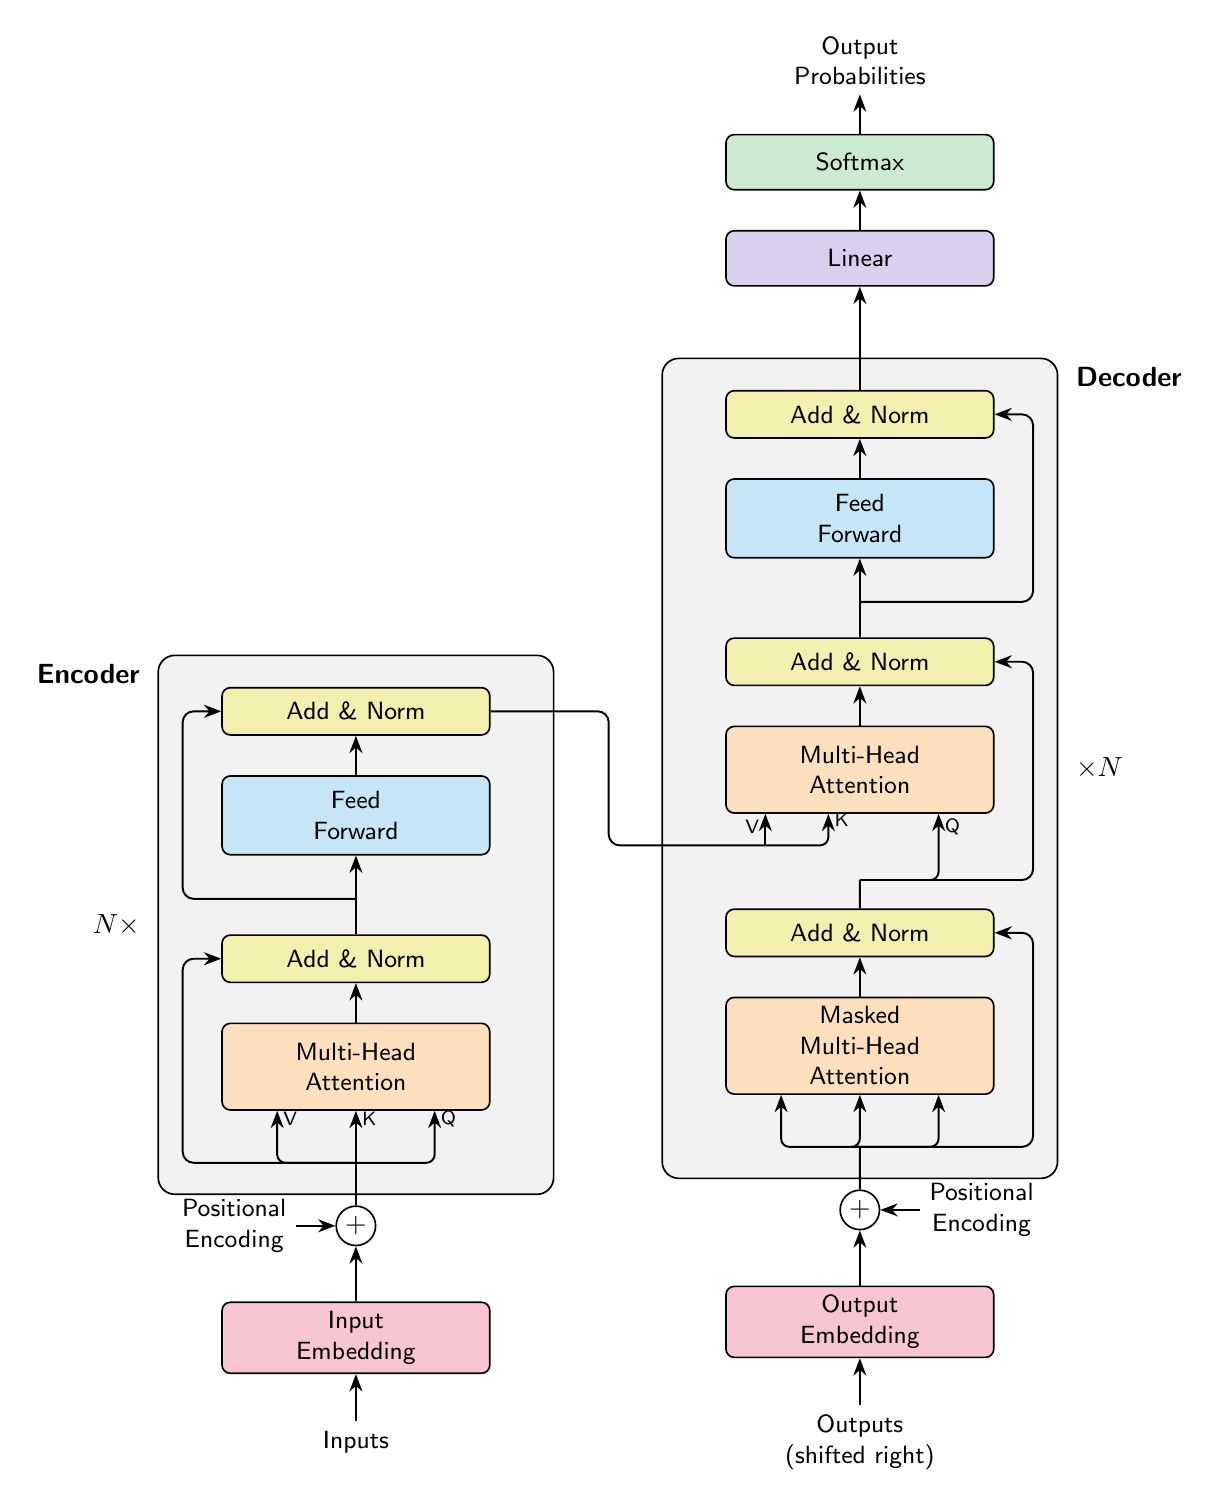
\begin{tikzpicture}

% ---------------- Encoder ----------------
\node[io] (ein) at (0,0) {Inputs};
\node[embed, above=6mm of ein] (eemb) {Input\\Embedding};
\node[pe, above=7mm of eemb] (eadd) {$+$};
\node[io, left=5mm of eadd] (epe) {Positional\\Encoding};
\node[attn, above=12mm of eadd] (eatt) {Multi-Head\\Attention};
\node[norm, above=5mm of eatt] (en1) {Add \& Norm};
\node[ffn, above=10mm of en1] (effn) {Feed\\Forward};
\node[norm, above=5mm of effn] (en2) {Add \& Norm};

\coordinate (eb1) at ($(eadd.north)!0.45!(eatt.south)$);
\coordinate (eb2) at ($(en1.north)!0.45!(effn.south)$);

\draw[flow] (ein) -- (eemb);
\draw[flow] (eemb) -- (eadd);
\draw[flow] (epe) -- (eadd);
\draw[line width=0.7pt] (eadd) -- (eb1);
\foreach \dx/\lbl in {-10mm/V, 0mm/K, 10mm/Q} {
  \draw[flow, rounded corners=3pt] (eb1) -| ($(eatt.south)+(\dx,0)$)
    node[pos=0.92, right=-0.5mm, font=\sffamily\scriptsize] {\lbl};
}
\draw[res] (eb1) -- ++(-22mm,0) |- (en1.west);
\draw[flow] (eatt) -- (en1);
\draw[flow] (en1) -- (effn);
\draw[res] (eb2) -- ++(-22mm,0) |- (en2.west);
\draw[flow] (effn) -- (en2);

\begin{scope}[on background layer]
  \node[stack, fit=(eb1)(eatt)(en2)] (estack) {};
\end{scope}
\node[left=1mm of estack.west, font=\sffamily\normalsize] {$N\times$};
\node[anchor=north east, font=\sffamily\bfseries] at ($(estack.north west)+(-1mm,0)$) {Encoder};

% ---------------- Decoder ----------------
\node[io] (din) at (64mm,0) {Outputs\\(shifted right)};
\node[embed, above=6mm of din] (demb) {Output\\Embedding};
\node[pe, above=7mm of demb] (dadd) {$+$};
\node[io, right=5mm of dadd] (dpe) {Positional\\Encoding};
\node[attn, above=12mm of dadd] (datt) {Masked\\Multi-Head\\Attention};
\node[norm, above=5mm of datt] (dn1) {Add \& Norm};
\node[attn, above=12mm of dn1] (dx) {Multi-Head\\Attention};
\node[norm, above=5mm of dx] (dn2) {Add \& Norm};
\node[ffn, above=10mm of dn2] (dffn) {Feed\\Forward};
\node[norm, above=5mm of dffn] (dn3) {Add \& Norm};

\coordinate (db1) at ($(dadd.north)!0.45!(datt.south)$);
\coordinate (db2) at ($(dn1.north)!0.3!(dx.south)$);
\coordinate (db3) at ($(dn2.north)!0.45!(dffn.south)$);

\draw[flow] (din) -- (demb);
\draw[flow] (demb) -- (dadd);
\draw[flow] (dpe) -- (dadd);
\draw[line width=0.7pt] (dadd) -- (db1);
\foreach \dx in {-10mm, 0mm, 10mm} {
  \draw[flow, rounded corners=3pt] (db1) -| ($(datt.south)+(\dx,0)$);
}
\draw[res] (db1) -- ++(22mm,0) |- (dn1.east);
\draw[flow] (datt) -- (dn1);
\draw[line width=0.7pt] (dn1) -- (db2);
\draw[flow, rounded corners=3pt] (db2) -| ($(dx.south)+(10mm,0)$)
  node[pos=0.9, right=-0.5mm, font=\sffamily\scriptsize] {Q};
\draw[res] (db2) -- ++(22mm,0) |- (dn2.east);
\draw[flow] (dx) -- (dn2);
\draw[flow] (dn2) -- (dffn);
\draw[res] (db3) -- ++(22mm,0) |- (dn3.east);
\draw[flow] (dffn) -- (dn3);

% Cross-attention: encoder output feeds K and V of the decoder.
\coordinate (xk) at ($(dx.south)+(-12mm,-4mm)$);
\draw[line width=0.7pt, rounded corners=4pt] (en2.east) -- ++(15mm,0) |- (xk);
\draw[flow] (xk) -- ($(dx.south)+(-12mm,0)$) node[pos=0.6, left=-0.5mm, font=\sffamily\scriptsize] {V};
\draw[flow, rounded corners=3pt] (xk) -| ($(dx.south)+(-4mm,0)$) node[pos=0.9, right=-0.5mm, font=\sffamily\scriptsize] {K};

\begin{scope}[on background layer]
  \node[stack, fit=(db1)(datt)(dn3)] (dstack) {};
\end{scope}
\node[right=1mm of dstack.east, font=\sffamily\normalsize] {$\times N$};
\node[anchor=north west, font=\sffamily\bfseries] at ($(dstack.north east)+(1mm,0)$) {Decoder};

% ---------------- Output head ----------------
\node[lin, above=9mm of dstack.north] (lin) {Linear};
\node[soft, above=5mm of lin] (soft) {Softmax};
\node[io, above=5mm of soft] (prob) {Output\\Probabilities};
\draw[flow] (dn3.north) -- (lin);
\draw[flow] (lin) -- (soft);
\draw[flow] (soft) -- (prob);

\end{tikzpicture}
\end{document}
